% IEEE-format project report: Project 12, Systolic Array Matrix Multiplication Accelerator
% Compile: pdflatex main && bibtex-free (references are inline) -> pdflatex main (twice)
% On Overleaf: upload this folder (main.tex + figures/) and compile with pdfLaTeX.
\documentclass[conference]{IEEEtran}
\IEEEoverridecommandlockouts

\usepackage{cite}
\usepackage{amsmath,amssymb}
\usepackage{graphicx}
\usepackage{booktabs}
\usepackage{array}
\usepackage{url}
\usepackage[hidelinks]{hyperref}

\graphicspath{{figures/}}
\newcommand{\code}[1]{\texttt{#1}}

\begin{document}

\title{A 4$\times$4 Output-Stationary Systolic Array\\ for Signed 8-bit Matrix Multiplication}

\author{
\IEEEauthorblockN{Parrv, Raghav, Ranjeet, Abhijeet, Malhar}
\IEEEauthorblockA{Modern Computer Architecture, Project 12\\
B.Tech Computer Science \& Artificial Intelligence\\
[Institution Name], [City], India}
}

\maketitle

% ---------------------------------------------------------------------------
\begin{abstract}
Matrix multiplication dominates the arithmetic of neural-network inference, and
systolic arrays are the standard way to accelerate it in hardware. We present a
4$\times$4 output-stationary systolic array, written in synthesizable
Verilog-2005, that multiplies 8-bit signed matrices with 32-bit signed
accumulators. Skewed rows of $A$ and columns of $B$ flow through a grid of 16
multiply-accumulate (MAC) processing elements while a Moore controller
sequences clear, compute and drain phases. One multiplication completes in
11 clock cycles, against 64 for a one-MAC sequential baseline with the same
interface (5.82$\times$ fewer cycles), and both designs match a NumPy golden
model on all 10 test cases. Implemented on a Xilinx Artix-7 (Basys~3) FPGA, the
array reaches 99.4\,MHz and delivers a 6.10$\times$ wall-clock speed-up over the
baseline for about 5$\times$ the look-up tables (LUTs).
\end{abstract}

\begin{IEEEkeywords}
systolic array, matrix multiplication, hardware accelerator, output-stationary
dataflow, FPGA, Verilog
\end{IEEEkeywords}

% ---------------------------------------------------------------------------
\section{Introduction}
The fully connected and convolution layers of a neural network reduce to large
matrix products~\cite{sze2017}. Computing $C = A \times B$ for two $N \times N$
matrices needs $N^3$ MAC operations; a datapath with a single MAC unit performs
them one after another, so even a 4$\times$4 product takes 64 cycles.

A \emph{systolic array} is a grid of identical processing elements (PEs) through
which data moves rhythmically, one PE per clock~\cite{kung1979,kung1982}. Each
PE multiplies the operands passing through it and adds the product to a local
sum. Because each operand is reused as it travels across a row or down a
column, many PEs work in the same cycle while each value is read from the input
buffers only once.

This report describes the design, verification and FPGA implementation of a
4$\times$4 output-stationary systolic array and compares it with a one-MAC
sequential baseline. Section~\ref{sec:lit} reviews related work,
Section~\ref{sec:prop} presents the proposed design, Section~\ref{sec:results}
reports verification and implementation results, and
Section~\ref{sec:contrib} lists individual contributions.

% ---------------------------------------------------------------------------
\section{Literature Review}\label{sec:lit}

\subsection{Origins of systolic arrays}
Kung and Leiserson introduced systolic arrays as a way to map regular
algorithms such as matrix multiplication and convolution onto VLSI: a network of
simple, locally connected cells through which data is ``pumped'' in a regular
rhythm~\cite{kung1979}. Kung later argued that the main benefit is balancing
computation with I/O bandwidth: an operand fetched once from memory is used by
many cells, so throughput grows with the number of cells without a matching
growth in memory traffic~\cite{kung1982}. S.~Y.~Kung formalised how to derive
such arrays from dependence graphs using space-time mappings~\cite{skung1988};
the input skew used in this project is a direct instance of that mapping.

\subsection{Dataflow taxonomy}
Chen \emph{et al.} classified deep-learning accelerators by which operand stays
in a PE: \emph{weight-stationary} (WS) keeps weights in place,
\emph{output-stationary} (OS) keeps partial sums in place, and
\emph{row-stationary} balances reuse of all three~\cite{chen2016}. Their Eyeriss
chip showed that the choice of dataflow, rather than the number of MACs, often
dominates energy efficiency~\cite{chen2017}. Sze \emph{et al.} survey these
trade-offs in detail~\cite{sze2017}. In an OS array each output never moves
until the end of the computation, so accumulators can be wide (32-bit here)
while the moving operands stay narrow (8-bit).

\subsection{Systolic arrays in modern accelerators}
Google's Tensor Processing Unit uses a 256$\times$256 systolic array of 8-bit
MACs (65,536 units) in a weight-stationary arrangement and reports large gains
in performance per watt over contemporary CPUs and GPUs for inference
workloads~\cite{jouppi2017}. SCALE-Sim, a cycle-accurate simulator for
systolic CNN accelerators, compares OS, WS and input-stationary mappings and
shows that the best dataflow depends on layer shape and array
size~\cite{samajdar2018}. Gemmini is an open-source generator that produces
systolic arrays supporting both OS and WS dataflows and integrates them with a
RISC-V system for full-stack evaluation~\cite{genc2021}. Xu \emph{et al.}
survey design and optimization techniques for systolic-array accelerators,
including dataflow choice, tiling and sparsity support~\cite{xu2023}.

\subsection{Number format and FPGA mapping}
Integer-only inference with 8-bit operands and 32-bit accumulators loses little
accuracy for common networks~\cite{jacob2018}, which motivates our choice of
\code{DW}~$=8$ and \code{AW}~$=32$. On Xilinx 7-series FPGAs, multipliers can
be built either from dedicated DSP48E1 slices~\cite{ug479} or from LUTs and
carry chains; the synthesis tool chooses unless directed
otherwise~\cite{ug901}.

\subsection{Positioning of this work}
Production arrays such as the TPU are large and weight-stationary. Our goal is
different: a small, fully verified OS array whose cycle-level behaviour can be
traced by hand, compared against a sequential baseline with an identical
interface, so that the speed-up and its hardware cost are measured on the same
tools, test vectors and FPGA.

% ---------------------------------------------------------------------------
\section{Proposed Solution}\label{sec:prop}

\subsection{System overview}
Fig.~\ref{fig:block} shows the top-level module \code{systolic\_top}. An
\code{input\_buffer} stores $A$ and $B$ and drives skewed values onto the left
and top edges of a 4$\times$4 \code{systolic\_array}. A \code{controller}
finite-state machine (FSM) sequences each run, and an \code{output\_collector}
reads any result. Table~\ref{tab:params} lists the parameters. All modules use
one clock, a synchronous active-high reset, and \code{signed} arithmetic.

\begin{figure*}[t]
  \centering
  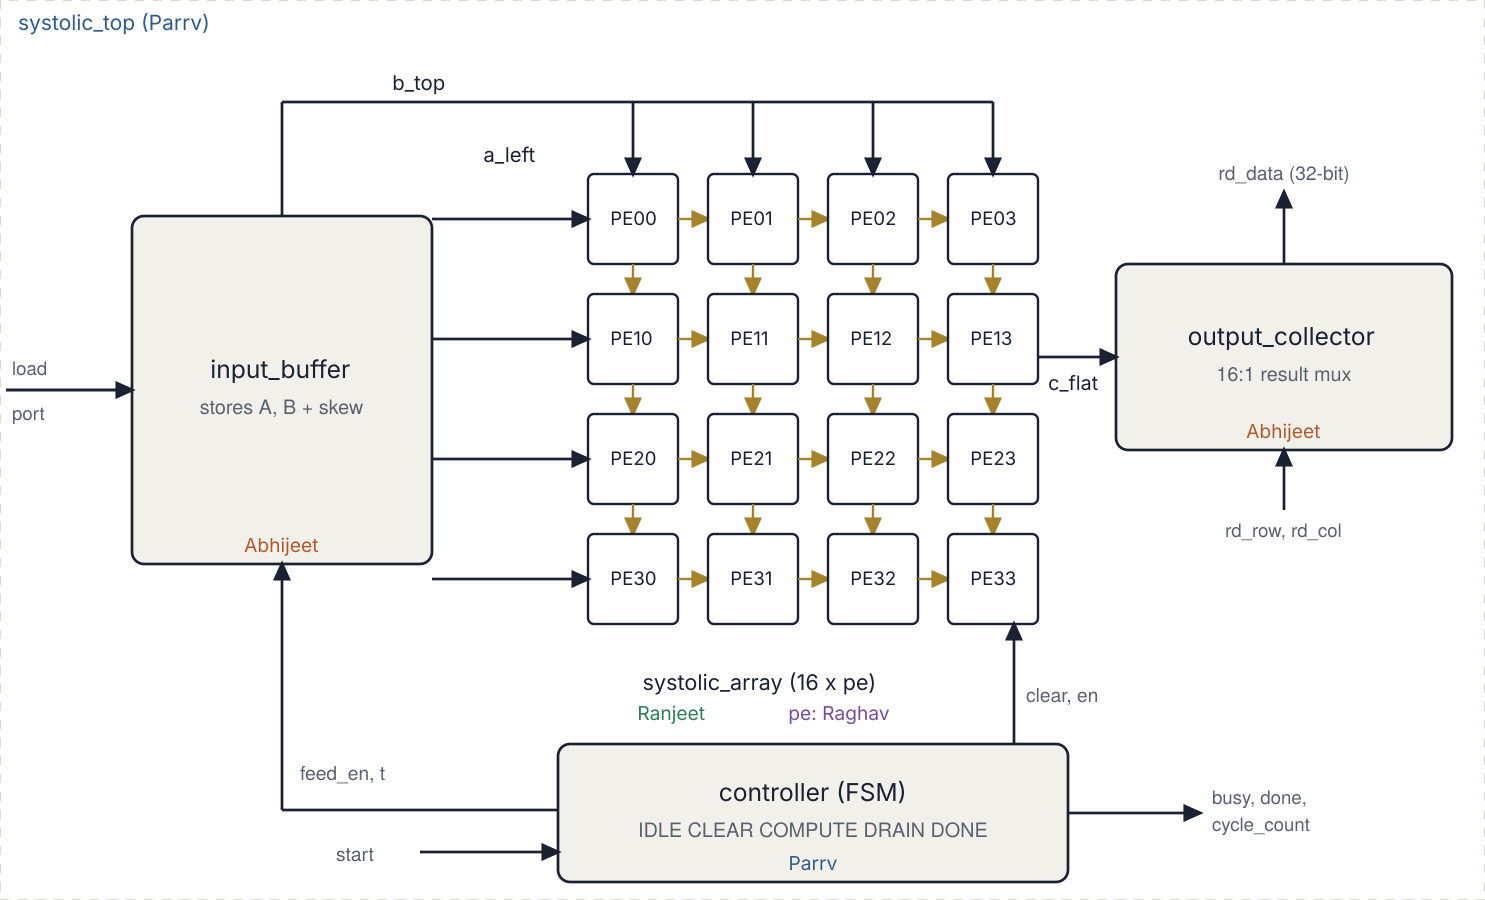
\includegraphics[width=0.72\textwidth]{block_diagram.png}
  \caption{Block diagram of \code{systolic\_top}. The input buffer feeds skewed
  rows of $A$ from the left and skewed columns of $B$ from the top; gold arrows
  are registered PE-to-PE links; the controller sequences clearing, feeding and
  draining; the output collector reads any result.}
  \label{fig:block}
\end{figure*}

\begin{table}[t]
  \centering
  \caption{Design Parameters}
  \label{tab:params}
  \footnotesize
  \begin{tabular}{@{}l l p{3.6cm}@{}}
    \toprule
    Param. & Value & Reason \\
    \midrule
    $N$  & 4 & 4$\times$4 array, 16 PEs \\
    \code{DW} & 8-bit signed & Range $-128$ to $127$ \\
    \code{AW} & 32-bit signed & Largest result $4\times(-128)^2 = 65{,}536$ needs 18 bits \\
    \code{TW} & 8 bits & Feed counter $t$ reaches 9 \\
    \bottomrule
  \end{tabular}
\end{table}

\subsection{Processing element}
Each PE performs, on every rising clock edge,
\begin{equation}
\begin{aligned}
a_{\text{out}} &\leftarrow a_{\text{in}}, \qquad b_{\text{out}} \leftarrow b_{\text{in}},\\
\text{acc} &\leftarrow
\begin{cases}
0 & \text{if } \code{clear},\\
\text{acc} + a_{\text{in}} \cdot b_{\text{in}} & \text{else if } \code{en},\\
\text{acc} & \text{otherwise.}
\end{cases}
\end{aligned}
\end{equation}
The pass-through registers update every cycle regardless of \code{en}, so data
keeps flowing through the array while accumulation is paused. The 8$\times$8
signed product is 16 bits wide and is sign-extended into the 32-bit
accumulator.

\subsection{Array and output-stationary dataflow}
Two nested \code{generate} loops instantiate 16 PEs. Two 2-D wire arrays carry
data between neighbours: \code{a\_bus[i][j]} is the $A$ value entering PE$(i,j)$
from the left and \code{b\_bus[i][j]} the $B$ value entering from above. PE$(i,j)$
drives its registered \code{a\_out} onto \code{a\_bus[i][j+1]} and \code{b\_out}
onto \code{b\_bus[i+1][j]}. Row $i$ of $A$ therefore moves right and column $j$
of $B$ moves down, exactly one PE per clock, while PE$(i,j)$ accumulates
\begin{equation}
C_{ij} = \sum_{k=0}^{N-1} A_{ik}\,B_{kj}
\end{equation}
in place. The 16 accumulators are exposed on a flattened 512-bit bus, with
$C_{ij}$ at bits \code{(i*N+j)*AW +: AW}, because Verilog-2005 has no array
ports. The array has no control logic of its own: \code{clear} and \code{en}
are broadcast to all PEs.

\subsection{Input skew}
For PE$(i,j)$ to multiply a matching pair, $A_{ik}$ and $B_{kj}$ must arrive in
the same cycle. $A_{ik}$ travels $j$ PEs right and $B_{kj}$ travels $i$ PEs
down, so row $i$ of $A$ is delayed by $i$ cycles and column $j$ of $B$ by $j$
cycles. For feed cycle $t$:
\begin{equation}
\begin{aligned}
\code{a\_left}_i &= A_{i,\,t-i} \quad \text{if } 0 \le t-i < N, \text{ else } 0,\\
\code{b\_top}_j  &= B_{t-j,\,j} \quad \text{if } 0 \le t-j < N, \text{ else } 0.
\end{aligned}
\end{equation}
$A_{ik}$ then enters at cycle $i+k$ and reaches column $j$ at $i+j+k$; $B_{kj}$
enters at $j+k$ and reaches row $i$ at the same cycle. Every pair meets at
\begin{equation}
t = i + j + k,
\end{equation}
so the first product occurs in PE$(0,0)$ at $t=0$ and the last in PE$(3,3)$ at
$t = 3N-3 = 9$. Table~\ref{tab:skew} shows the resulting staircase. The input
buffer implements this as a combinational multiplexer indexed by $t$, rather
than as shift-register delay chains, and outputs zeros when \code{feed\_en} is
low.

\begin{table}[t]
  \centering
  \caption{Values Entering the Array at Feed Cycle $t$ ($A_{12}$ = $A[1][2]$)}
  \label{tab:skew}
  \footnotesize
  \setlength{\tabcolsep}{3pt}
  \begin{tabular}{@{}c cccc cccc@{}}
    \toprule
    & \multicolumn{4}{c}{\code{a\_left} row} & \multicolumn{4}{c}{\code{b\_top} column}\\
    \cmidrule(lr){2-5}\cmidrule(l){6-9}
    $t$ & 0 & 1 & 2 & 3 & 0 & 1 & 2 & 3 \\
    \midrule
    0 & $A_{00}$ & 0 & 0 & 0 & $B_{00}$ & 0 & 0 & 0 \\
    1 & $A_{01}$ & $A_{10}$ & 0 & 0 & $B_{10}$ & $B_{01}$ & 0 & 0 \\
    2 & $A_{02}$ & $A_{11}$ & $A_{20}$ & 0 & $B_{20}$ & $B_{11}$ & $B_{02}$ & 0 \\
    3 & $A_{03}$ & $A_{12}$ & $A_{21}$ & $A_{30}$ & $B_{30}$ & $B_{21}$ & $B_{12}$ & $B_{03}$ \\
    4 & 0 & $A_{13}$ & $A_{22}$ & $A_{31}$ & 0 & $B_{31}$ & $B_{22}$ & $B_{13}$ \\
    5 & 0 & 0 & $A_{23}$ & $A_{32}$ & 0 & 0 & $B_{32}$ & $B_{23}$ \\
    6 & 0 & 0 & 0 & $A_{33}$ & 0 & 0 & 0 & $B_{33}$ \\
    7--9 & 0 & 0 & 0 & 0 & 0 & 0 & 0 & 0 \\
    \bottomrule
  \end{tabular}
\end{table}

\subsection{Controller}
A Moore FSM sequences each multiplication (Table~\ref{tab:fsm}). CLEAR zeroes
all 16 accumulators in one cycle. COMPUTE lasts $2N-1 = 7$ cycles, the window
in which some skewed input is non-zero. DRAIN lasts $N-1 = 3$ more cycles so
the last operands reach PE$(3,3)$; \code{en} therefore stays high for $3N-2 =
10$ cycles. All outputs are decoded from the state register, so they change
exactly on state boundaries. Accepting \code{start} in DONE allows
back-to-back multiplications without a reset, and because \code{en} drops in
DONE the results stay valid until the next \code{start}. One multiplication
takes $1+7+3 = 11$ cycles from \code{start} to \code{done}.

\begin{table}[t]
  \centering
  \caption{Controller States}
  \label{tab:fsm}
  \footnotesize
  \setlength{\tabcolsep}{4pt}
  \begin{tabular}{@{}l c c l@{}}
    \toprule
    State & Cycles & $t$ & Outputs high \\
    \midrule
    IDLE    & until \code{start} & -- & -- \\
    CLEAR   & 1 & -- & \code{clear}, \code{busy} \\
    COMPUTE & 7 ($2N-1$) & 0--6 & \code{feed\_en}, \code{en}, \code{busy} \\
    DRAIN   & 3 ($N-1$) & 7--9 & \code{en}, \code{busy} \\
    DONE    & until \code{start} & -- & \code{done} \\
    \bottomrule
  \end{tabular}
\end{table}

\subsection{Host interface and sequential baseline}
While \code{busy} is low, the host writes the 32 elements of $A$ and $B$ one
per clock through a load port (\code{load\_sel}, \code{load\_row},
\code{load\_col}, \code{load\_data}), pulses \code{start}, waits for
\code{done}, and reads $C_{rc}$ combinationally by setting \code{rd\_row} and
\code{rd\_col}. The baseline \code{sequential\_mac} has exactly the same ports
but a single MAC unit that iterates over $i$, $j$, $k$, taking $N^3 = 64$
cycles.

% ---------------------------------------------------------------------------
\section{Verification and Results}\label{sec:results}

\subsection{Verification method}
A NumPy golden model (seed 42) generates 10 test cases and computes each
product with 64-bit integers, written as row-major hex files. Every module has
a self-checking Icarus Verilog testbench that changes inputs on the falling
clock edge and prints PASS/FAIL. The top-level testbench loads each case through
the real load port, pulses \code{start}, waits for \code{done} and compares all
16 results; the baseline is tested the same way. Table~\ref{tab:verif}
summarises the results; every check passes.

\begin{table}[t]
  \centering
  \caption{Verification Summary}
  \label{tab:verif}
  \footnotesize
  \setlength{\tabcolsep}{3pt}
  \begin{tabular}{@{}l p{3.9cm} r@{}}
    \toprule
    Testbench & What it checks & Result \\
    \midrule
    \code{tb\_pe} & Signed MAC, extremes, \code{clear} priority, hold, pass-through & 27/27 \\
    \code{tb\_array} & Identity, all-ones, random signed (skew applied by testbench) & 48/48 \\
    \code{tb\_input\_buffer} & Skew staircase $t=0..9$; zeros when \code{feed\_en}$=0$ & pass \\
    \code{tb\_output\_collector} & All 16 read positions incl.\ negatives & pass \\
    \code{tb\_controller} & State lengths 1/7/10/11, back-to-back, mid-run reset & 31/31 \\
    \code{tb\_top} & 10 golden-model cases, end to end & 160/160 \\
    \code{tb\_sequential} & Same 10 cases on the baseline & 160/160 \\
    \bottomrule
  \end{tabular}
\end{table}

The 10 cases include identity$\times$random (checks the data path element by
element), all zeros, and the three extreme cases $127\times127$,
$(-128)\times(-128)$ and $127\times(-128)$, which produce the largest positive
(65,536) and most negative ($-65{,}024$) results and confirm signed arithmetic
end to end. The array testbench drives the array directly, isolating wiring
bugs from skew or FSM bugs; deliberately mis-wiring \code{b\_out} made 36 of
its 48 checks fail, confirming that it detects propagation errors.

Fig.~\ref{fig:wave} shows the diagonal wavefront in simulation: each value
appears at the next PE exactly one clock later, PE$(0,0)$ finishes $C_{00}$ at
$t=3$ and PE$(3,3)$ finishes $C_{33}$ at $t=9$. Fig.~\ref{fig:top} shows a full
run with load, one-cycle \code{start}, 11 busy cycles and \code{done}.

\begin{figure}[t]
  \centering
  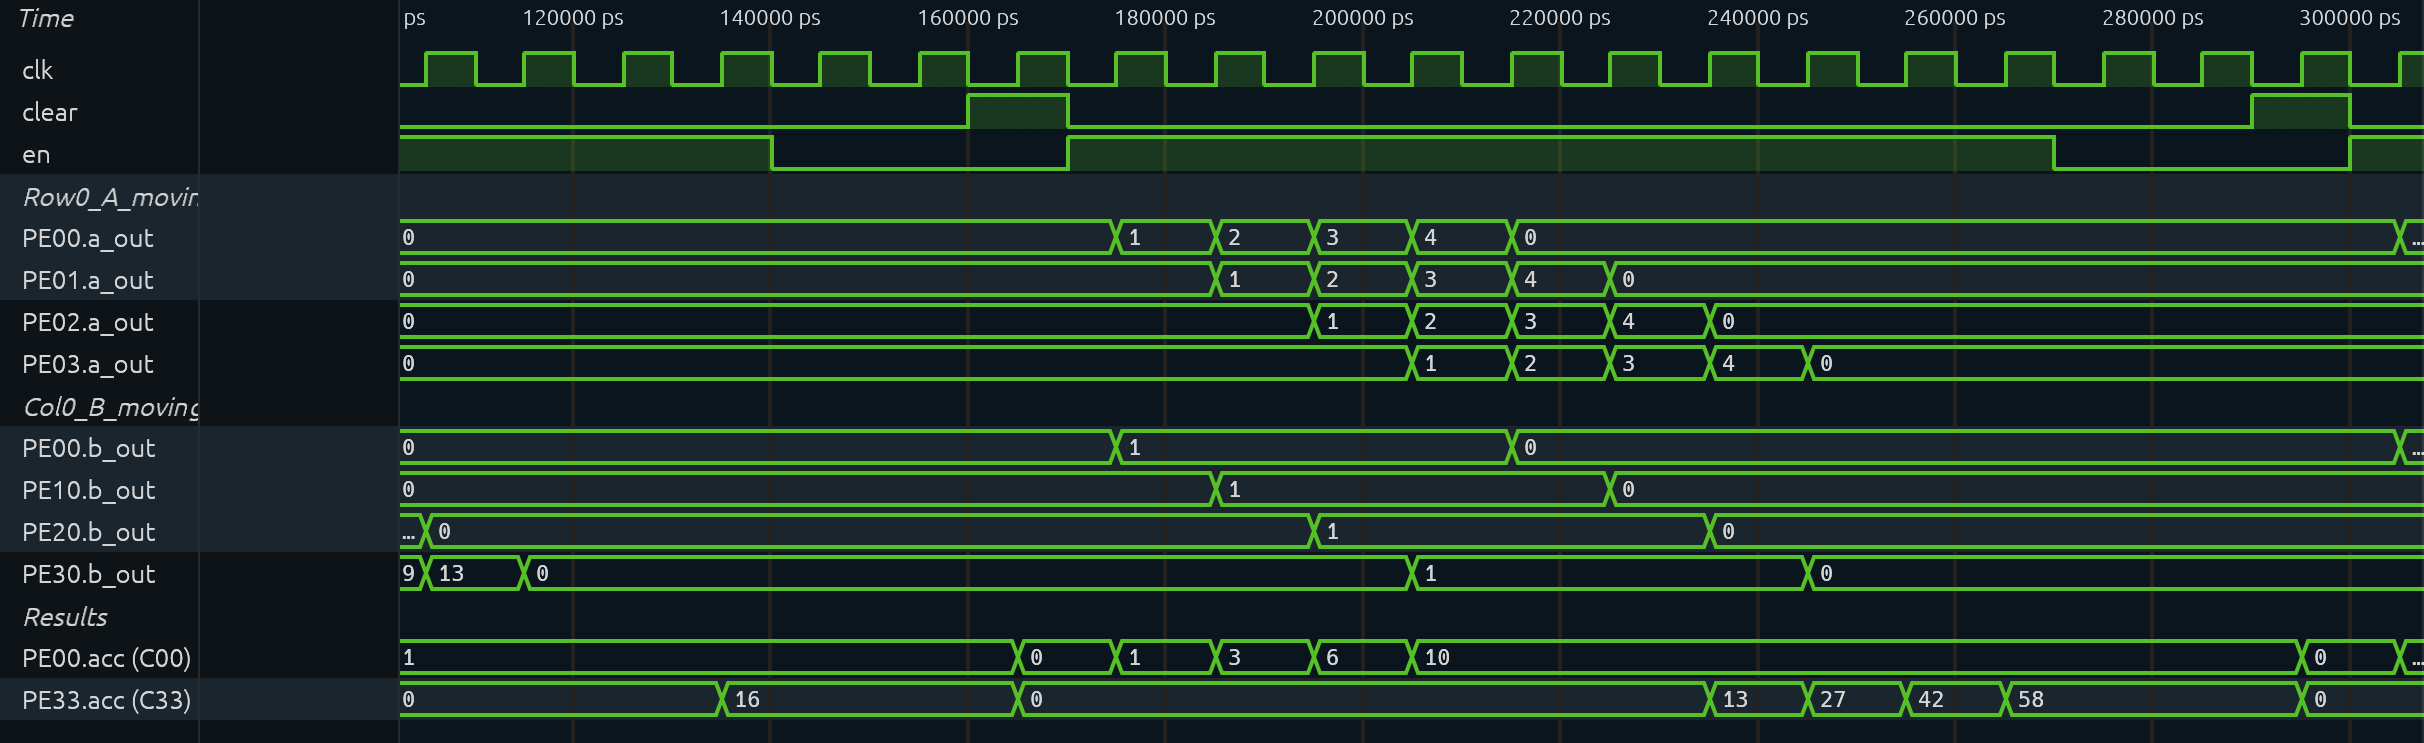
\includegraphics[width=\columnwidth]{array_wavefront.png}
  \caption{Array wavefront (all-ones $B$, $A$ = 1..16). Top: \code{a\_out}
  of PE$(0,0)$..PE$(0,3)$ (A moving right). Middle: \code{b\_out} of
  PE$(0,0)$..PE$(3,0)$ (B moving down). Bottom: accumulators of PE$(0,0)$ and
  PE$(3,3)$, offset by six cycles.}
  \label{fig:wave}
\end{figure}

\begin{figure*}[t]
  \centering
  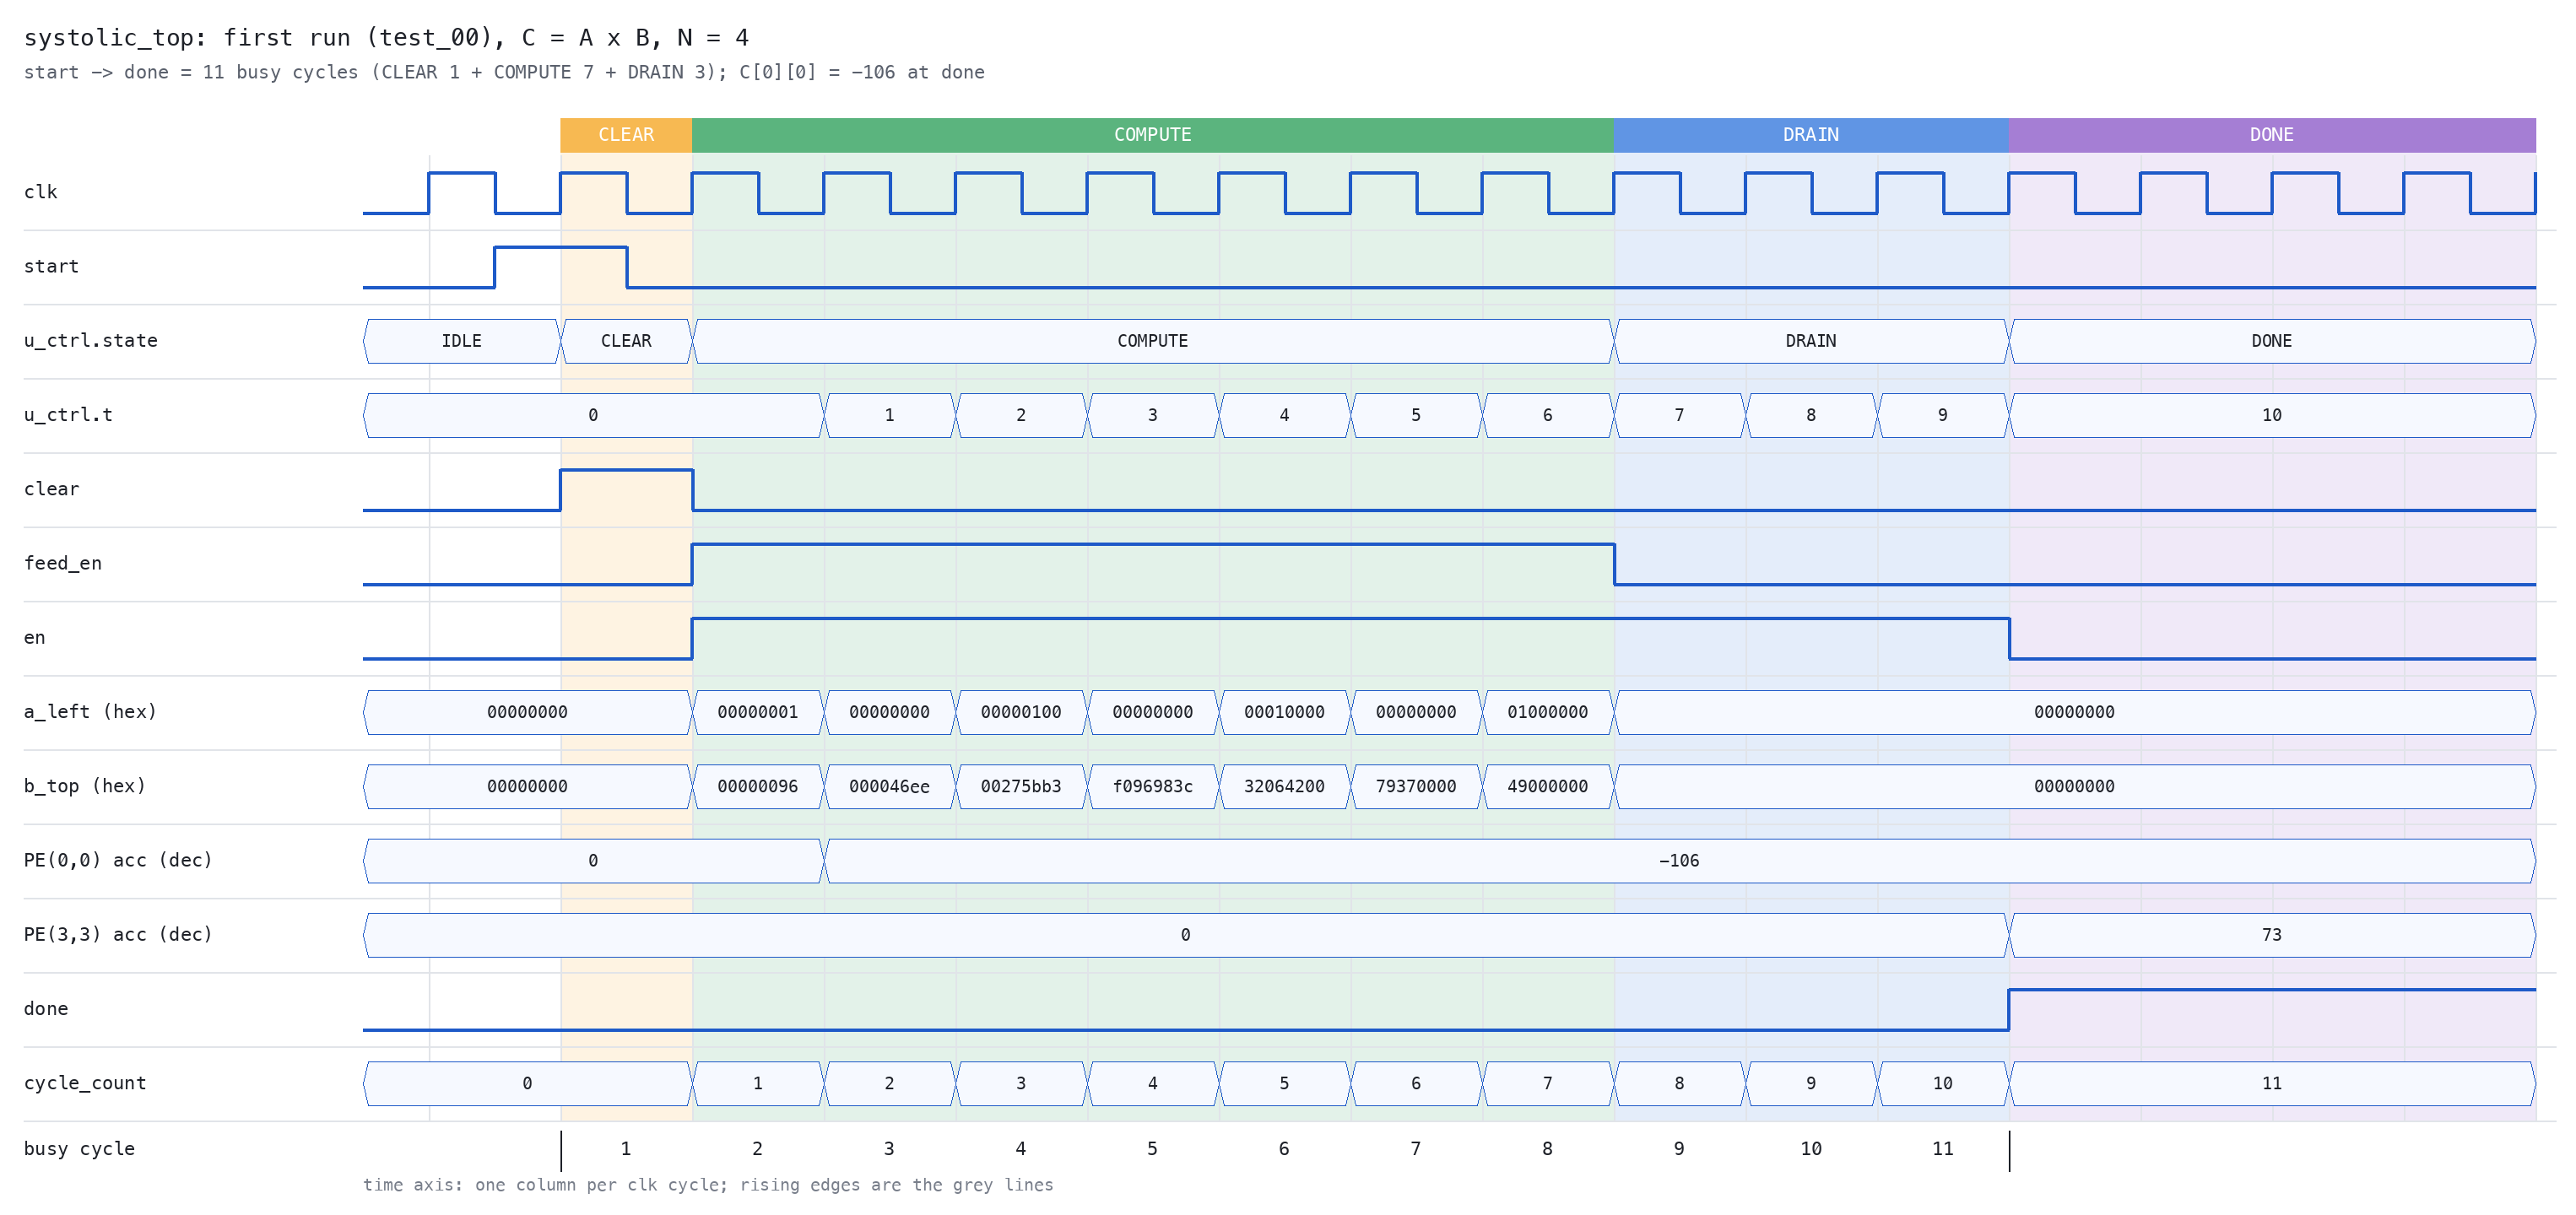
\includegraphics[width=0.85\textwidth]{top_run.png}
  \caption{Full-system run of test\_00: \code{start}, CLEAR (1 cycle), COMPUTE
  (7), DRAIN (3), then \code{done} with \code{cycle\_count} = 11.}
  \label{fig:top}
\end{figure*}

\subsection{Performance}
The systolic design needs $3N-2$ compute cycles plus one clear cycle; the
baseline needs $N^3$ (Table~\ref{tab:perf}). At $N=4$ this is 11 versus 64
cycles, confirmed in simulation by \code{cycle\_count} on all 10 tests. The
array averages $64/10 = 6.4$ MACs per compute cycle, with up to 12 of its 16
PEs active at once ($t = 4, 5$). Because the gap grows as $N^3/(3N-1)$, the
speed-up rises to about $22\times$ at $N=8$ and $87\times$ at $N=16$
(Fig.~\ref{fig:speedup}).

\begin{table}[t]
  \centering
  \caption{Cycle Count Versus Array Size}
  \label{tab:perf}
  \footnotesize
  \begin{tabular}{@{}r r r r@{}}
    \toprule
    $N$ & Systolic ($3N-1$) & Sequential ($N^3$) & Speed-up \\
    \midrule
    2  & 5  & 8    & 1.6$\times$ \\
    4  & 11 & 64   & 5.8$\times$ \\
    8  & 23 & 512  & 22.3$\times$ \\
    16 & 47 & 4096 & 87.1$\times$ \\
    \bottomrule
  \end{tabular}
\end{table}

\begin{figure}[t]
  \centering
  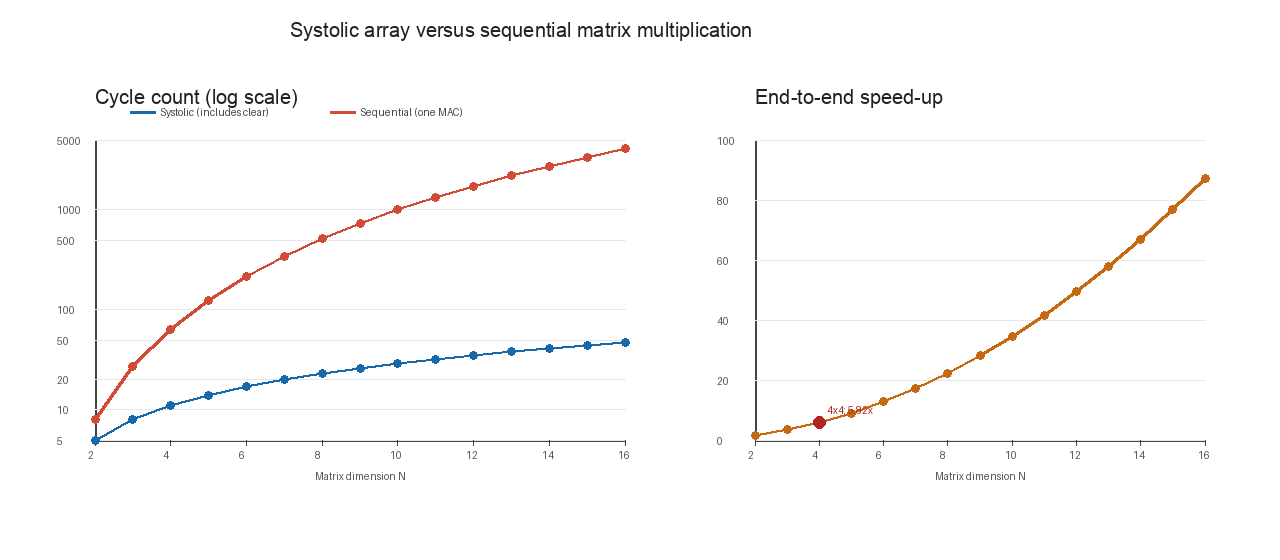
\includegraphics[width=\columnwidth]{speedup.png}
  \caption{Cycle count (log scale) and end-to-end speed-up versus array size
  $N$; the marked point is the implemented 4$\times$4 design.}
  \label{fig:speedup}
\end{figure}

\subsection{FPGA implementation}
Both designs were synthesized, placed and routed out of context with AMD Vivado
2026.1 for the Artix-7 \code{xc7a35tcpg236-1} (Basys~3) with a 10\,ns
(100\,MHz) clock constraint. Table~\ref{tab:synth} gives the results, with
$F_{\max} = 1000/(10 - \text{WNS})$\,MHz.

\begin{table}[t]
  \centering
  \caption{Implementation Results on Artix-7 xc7a35t}
  \label{tab:synth}
  \footnotesize
  \setlength{\tabcolsep}{4pt}
  \begin{tabular}{@{}l r r r@{}}
    \toprule
    Metric & Systolic & Sequential & Ratio \\
    \midrule
    LUTs & 1,940 (9.3\%) & 390 (1.9\%) & 4.97$\times$ \\
    Flip-flops & 987 (2.4\%) & 825 (2.0\%) & 1.20$\times$ \\
    DSP / BRAM & 0 / 0 & 0 / 0 & -- \\
    WNS (ns) & $-0.057$ & $-0.537$ & -- \\
    $F_{\max}$ (MHz) & 99.4 & 94.9 & -- \\
    Cycles per multiply & 11 & 64 & 5.82$\times$ fewer \\
    Time per multiply & 110.6\,ns & 674.4\,ns & 6.10$\times$ faster \\
    \bottomrule
  \end{tabular}
\end{table}

The flip-flop count matches the RTL: 512 accumulator bits plus 192
pass-through bits in the array (Vivado removed the unused \code{a\_out} of
column 3 and \code{b\_out} of row 3), 256 bits of $A$/$B$ storage, and 27
controller bits. Vivado built all multipliers from LUTs and carry chains rather
than DSP48E1 slices, which explains most of the 5$\times$ LUT cost. The systolic
critical path (10.035\,ns) runs from the controller's $t$ register through the
input buffer's skew multiplexer into the multiplier and adder of PE$(0,1)$;
every PE-to-PE link is registered, so the array itself is not the limit. Since
both designs run at nearly the same frequency, the 5.82$\times$ cycle advantage
becomes a 6.10$\times$ wall-clock speed-up.

% ---------------------------------------------------------------------------
\section{Individual Contributions}\label{sec:contrib}
Each member owned specific source files and wrote the report section on them;
no member edited another member's files. Table~\ref{tab:contrib} lists the
contributions.

\begin{table}[t]
  \centering
  \caption{Individual Contributions}
  \label{tab:contrib}
  \footnotesize
  \begin{tabular}{@{}l p{6.0cm}@{}}
    \toprule
    Member & Contribution \\
    \midrule
    Parrv & Controller FSM (\code{controller.v}) and top-level integration
            (\code{systolic\_top.v}); controller and full-system testbenches;
            block diagram; report integration (Introduction, Architecture,
            Conclusion). \\
    Raghav & Signed MAC processing element (\code{pe.v}) and its 27-check
             testbench; PE waveform evidence and demo presentation. \\
    Ranjeet & 4$\times$4 array wiring with \code{generate} loops
              (\code{systolic\_array.v}); 48-check array testbench and
              wavefront waveform; Vivado synthesis flow, constraints and
              timing/utilization analysis. \\
    Abhijeet & Input buffer with skew logic (\code{input\_buffer.v}) and
               output collector (\code{output\_collector.v}); their
               testbenches and skew-staircase waveform. \\
    Malhar & NumPy golden model and 10 test vectors; sequential MAC baseline
             (\code{sequential\_mac.v}) and its testbench; performance
             analysis and speed-up plot. \\
    \bottomrule
  \end{tabular}
\end{table}

% ---------------------------------------------------------------------------
\section{Conclusion and Future Work}
We designed, verified and implemented a 4$\times$4 output-stationary systolic
array for signed 8-bit matrix multiplication. It completes one multiplication
in 11 cycles, matches the golden model on all 10 test cases, and on an Artix-7
FPGA is 6.10$\times$ faster in wall-clock time than a one-MAC baseline for
about 5$\times$ the LUTs.

The main limitations are serial loading (32 cycles for $A$ and $B$, which
dominates end-to-end time for a single 4$\times$4 product), a fixed 4$\times$4
problem size, and no saturation or scaling for quantized layers. Future work
includes registering the input-buffer outputs to close timing above 100\,MHz,
mapping the multipliers to DSP48E1 slices, double-buffering $A$ and $B$ to
overlap loading with computation, scaling the parameterised RTL to 8$\times$8
or 16$\times$16, tiling larger matrices, and exploring a weight-stationary
variant as used in the TPU~\cite{jouppi2017}.

% ---------------------------------------------------------------------------
\begin{thebibliography}{99}

\bibitem{kung1979}
H.~T. Kung and C.~E. Leiserson, ``Systolic arrays (for VLSI),'' in
\emph{Sparse Matrix Proceedings 1978}, I.~S. Duff and G.~W. Stewart, Eds.
Philadelphia, PA, USA: SIAM, 1979, pp.~256--282.

\bibitem{kung1982}
H.~T. Kung, ``Why systolic architectures?'' \emph{Computer}, vol.~15, no.~1,
pp.~37--46, Jan. 1982.

\bibitem{skung1988}
S.~Y. Kung, \emph{VLSI Array Processors}. Englewood Cliffs, NJ, USA:
Prentice Hall, 1988.

\bibitem{chen2016}
Y.-H. Chen, J.~Emer, and V.~Sze, ``Eyeriss: A spatial architecture for
energy-efficient dataflow for convolutional neural networks,'' in \emph{Proc.
43rd Annu. Int. Symp. Comput. Archit. (ISCA)}, 2016, pp.~367--379.

\bibitem{chen2017}
Y.-H. Chen, T.~Krishna, J.~S. Emer, and V.~Sze, ``Eyeriss: An energy-efficient
reconfigurable accelerator for deep convolutional neural networks,''
\emph{IEEE J. Solid-State Circuits}, vol.~52, no.~1, pp.~127--138, Jan. 2017.

\bibitem{sze2017}
V.~Sze, Y.-H. Chen, T.-J. Yang, and J.~S. Emer, ``Efficient processing of deep
neural networks: A tutorial and survey,'' \emph{Proc. IEEE}, vol.~105,
no.~12, pp.~2295--2329, Dec. 2017.

\bibitem{jouppi2017}
N.~P. Jouppi \emph{et al.}, ``In-datacenter performance analysis of a tensor
processing unit,'' in \emph{Proc. 44th Annu. Int. Symp. Comput. Archit.
(ISCA)}, 2017, pp.~1--12.

\bibitem{samajdar2018}
A.~Samajdar, Y.~Zhu, P.~Whatmough, M.~Mattina, and T.~Krishna, ``SCALE-Sim:
Systolic CNN accelerator simulator,'' 2018, \emph{arXiv:1811.02883}.

\bibitem{genc2021}
H.~Genc \emph{et al.}, ``Gemmini: Enabling systematic deep-learning
architecture evaluation via full-stack integration,'' in \emph{Proc. 58th
ACM/IEEE Design Autom. Conf. (DAC)}, 2021, pp.~769--774.

\bibitem{xu2023}
R.~Xu, S.~Ma, Y.~Guo, and D.~Li, ``A survey of design and optimization for
systolic array-based DNN accelerators,'' \emph{ACM Comput. Surv.}, vol.~56,
no.~1, Art. no.~20, 2023.

\bibitem{jacob2018}
B.~Jacob \emph{et al.}, ``Quantization and training of neural networks for
efficient integer-arithmetic-only inference,'' in \emph{Proc. IEEE/CVF Conf.
Comput. Vis. Pattern Recognit. (CVPR)}, 2018, pp.~2704--2713.

\bibitem{ug479}
Xilinx, Inc., ``7 Series DSP48E1 Slice User Guide,'' UG479.

\bibitem{ug901}
AMD, ``Vivado Design Suite User Guide: Synthesis,'' UG901.

\bibitem{verilog2005}
\emph{IEEE Standard for Verilog Hardware Description Language}, IEEE Std
1364-2005, 2006.

\bibitem{icarus}
S.~Williams, ``Icarus Verilog.'' [Online]. Available:
\url{https://steveicarus.github.io/iverilog/}

\end{thebibliography}

\end{document}
